\chapter{Zaključek in rezultati}

V tem poglavju si bomo pogledali metodo vizualizacije nevronske mreže in kakšne rezultate dobimo. Pri tem bomo sledili~\cite{Gabella_2021}.

Pri gradnji Mapper grafa iz nevronske mreže lahko za vsak sloj \(i\) z \(N_i\) nevroni, spremljamo evolucijo uteži nevronov, ki vstopajo vanj. Z drugimi besedami spremljamo stolpce v matriki uteži med nivojema \(i-1\) in \(i\). Nato pa za vsak korak v procesu učenja, ki ga izvedemo z metodo gradientnega spusta dobimo \(N_i\) vektorjev uteži velikosti \(N_{i-1}\), kar interpretiramo kot \(N_i\) točk v prostoru dimenzije \(N_{i-1}\). Ob koncu učenja dobimo oblak točk z \(\text{št.\ korakov} \times N_i\) točk, ki so dimenzije \(N_{i-1}\). Točke so nato s PCA projekcijo projicirane v 2-dimenzionalni prostor. Od tod potem z Mapper algoritmom zgradimo graf.

Rezultati, ki jih bomo predstavili so povzeti iz članka~\cite{Gabella_2021}. Pogledali si bomo Mapper graf nevronske mreže, ki je bila zgrajena na podatkovni zbirki MNIST.\ Gre za veliko podatkovno zbirko ročno napisanih števk (slik velikosti 28$\times$28), ki se pogosto uporablja za učenje in testiranje metod strojnega učenja.
Nevronska mreža ima dva skrita nivoja s 100 nevroni in sigmoidno aktivacijsko funkcijo. Začetne vrednosti uteži so bile nastavljene na naključne majhne vrednosti. Za filter funkcijo je bila uporabljena $L^2$ norma in DBSCAN kot algoritem gručenja.

\begin{figure}[H]
  \centering
  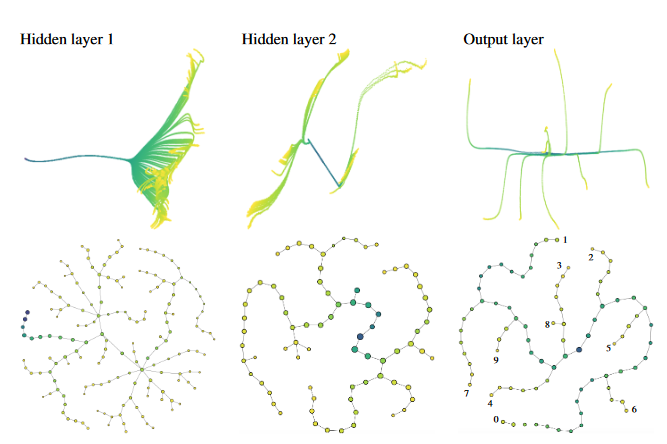
\includegraphics[width=1\linewidth]{resources/mapper-minst.png}
  \caption{Evolucija uteži učenja nevronske mreže. Vir:~\cite{Gabella_2021}}\label{fig:evolution}
\end{figure}

Z modro barvo so predstavljene uteži na začetku učenja in z rumeno na koncu. Opazimo, da se graf v zadnjem sloju razveji na 10 vej, kjer vsaka predstavlja eno izmed desetih števk. V skritem nivoju pa lahko opazimo, da se uteži nekaj časa razvijajo v enaki smeri in se šele nato razvejijo, kar bi lahko bila posledica PCA projekcije. Omenimo še, da so smeri razvejanja v različnih poskusih učenja ostale skoraj konstantne. V zadnjem sloju opazimo, da se graf že na začetku usmeri na dve nasprotni veji, ki se nato še dalje razvejita. Vidno je tudi, da so si nekatere števke zelo podobne, recimo osmica in trojka sta si zelo sorodni.
